\documentclass[titlepage]{article}
\usepackage{graphicx}
\usepackage{wrapfig}
\usepackage{enumitem}% http://ctan.org/pkg/enumitem
\graphicspath{ {./img/} }

\author{Jeffrey Meyer \and Bayli Boston}
\title{Theory of Computer Sciece: Homework \#4 - NandToTetris | Memory}

\begin{document}

\maketitle

\newpage

\section{Project 3}

\begin{enumerate}
  \item[a)]{
    \begin{description}
      \item[Bit]{
        All test passed

        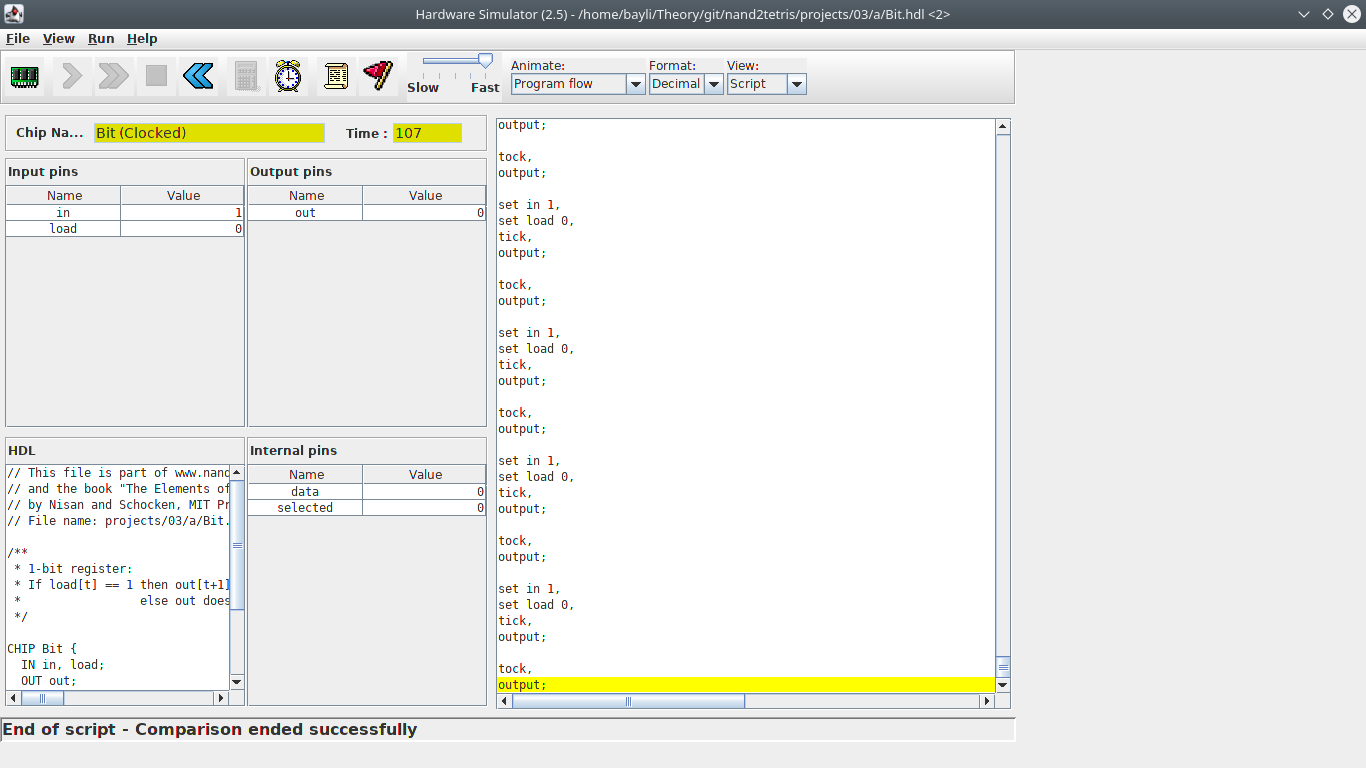
\includegraphics[width=.9\textwidth]{a/Bit.png}
      }
      \item[Register]{
        All test passed

        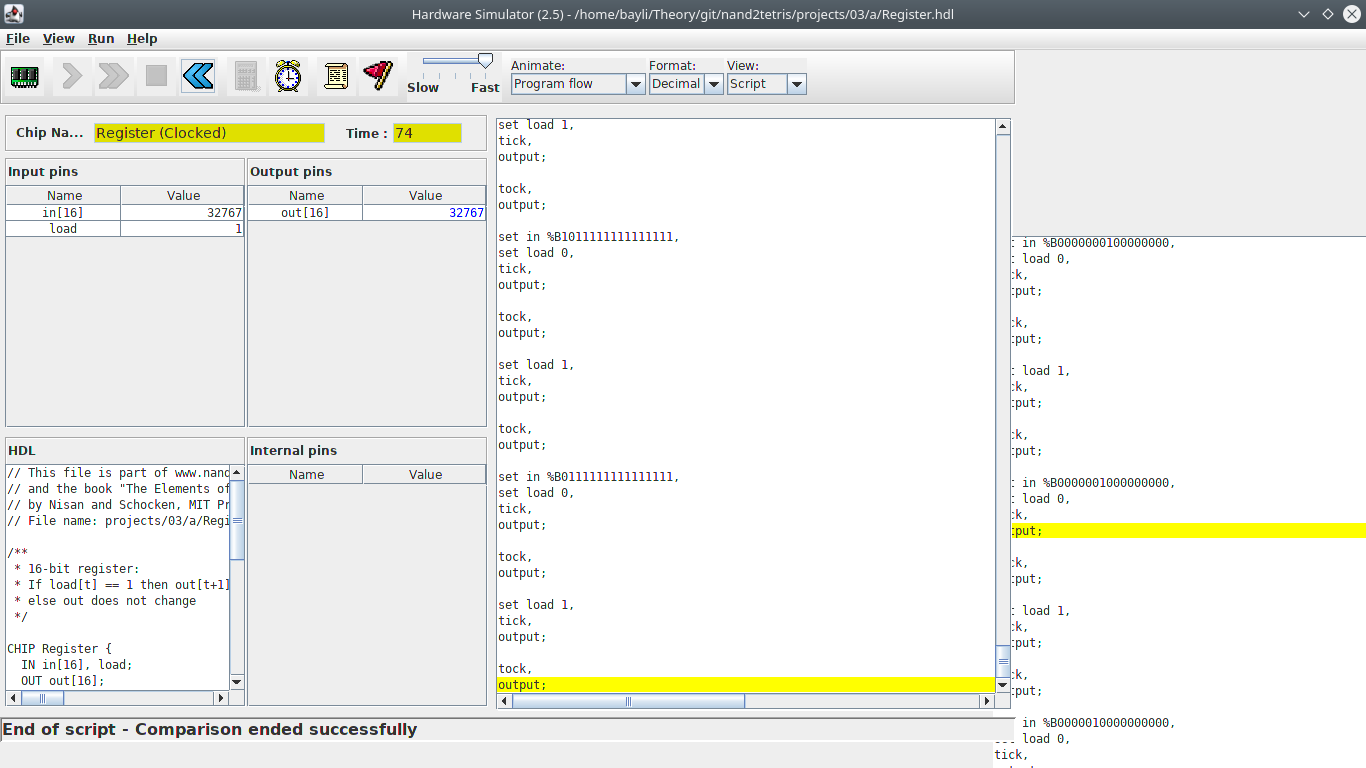
\includegraphics[width=.9\textwidth]{a/Register.png}
      }
      \item[RAM8]{
        All test passed

        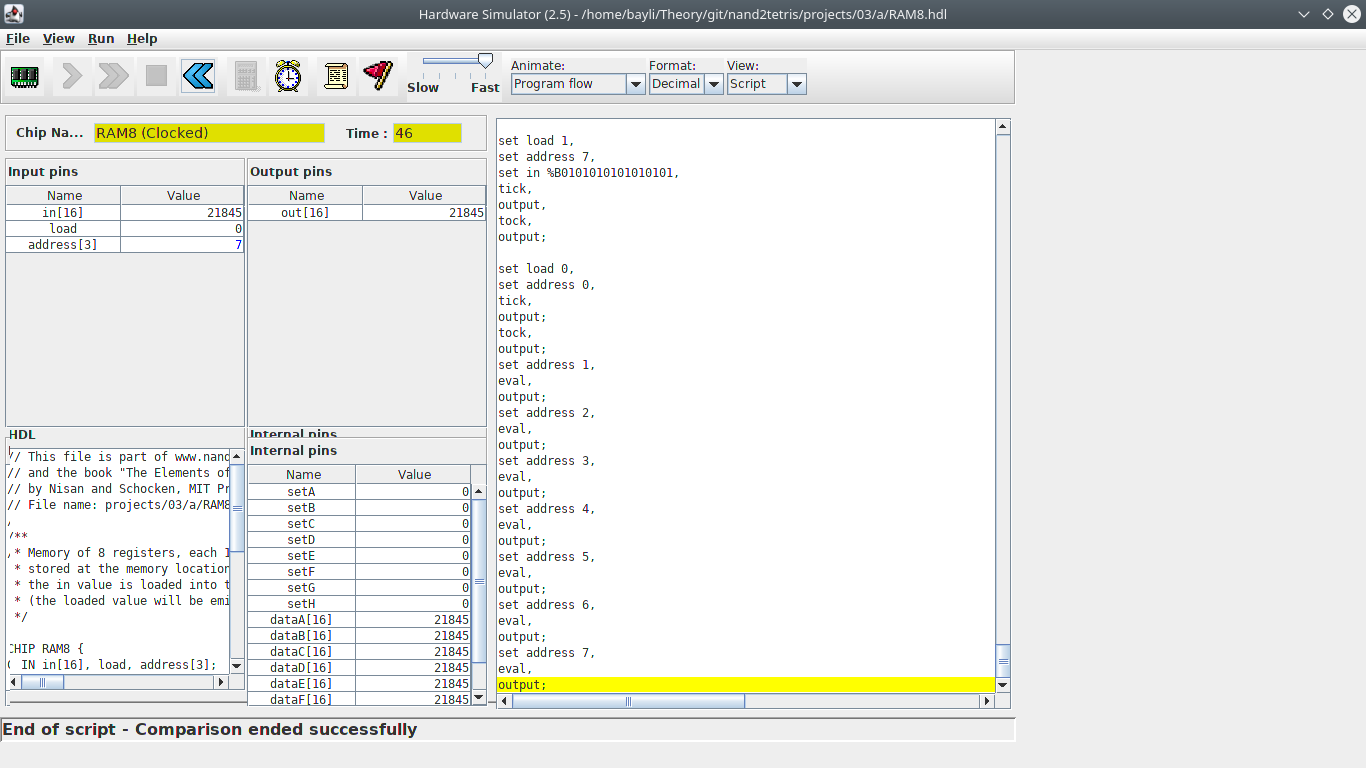
\includegraphics[width=.9\textwidth]{a/RAM8.png}
      }
      \item[RAM64]{
        All test passed

        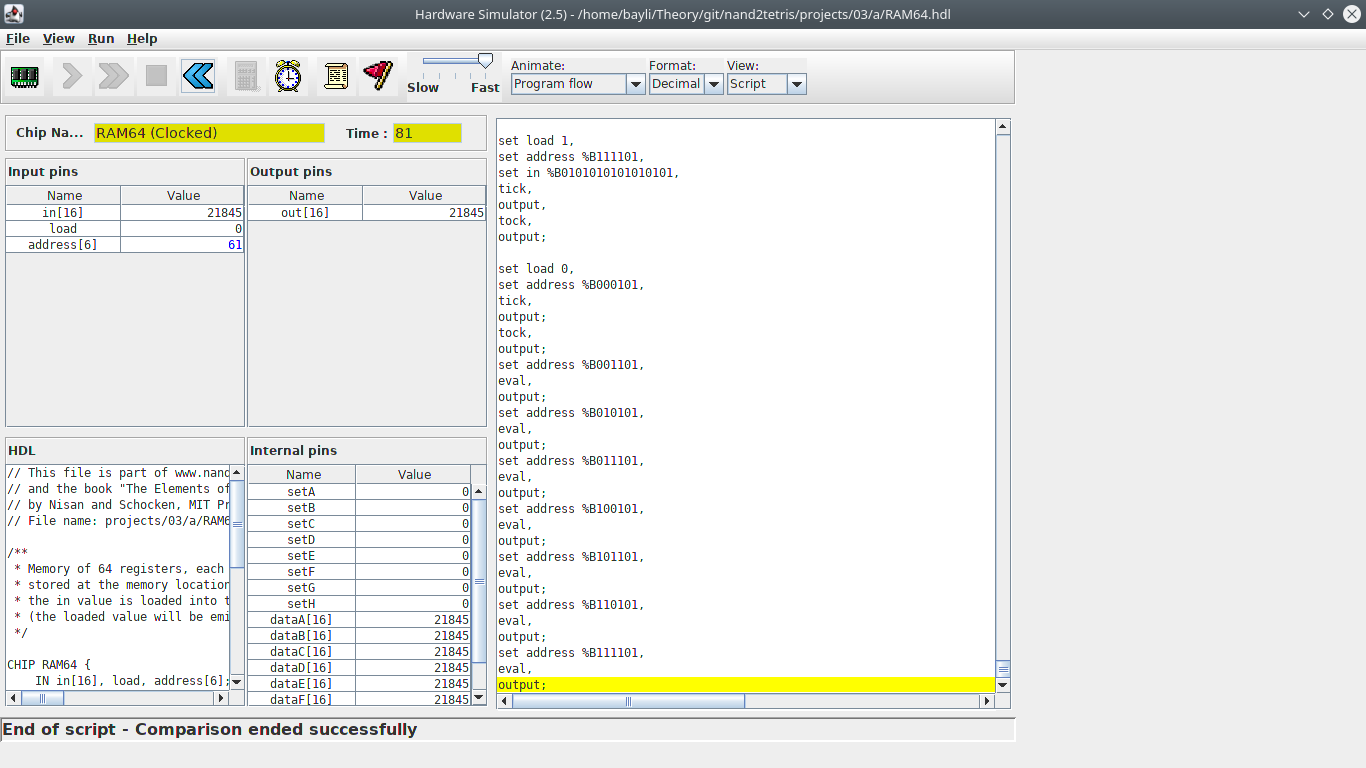
\includegraphics[width=.9\textwidth]{a/RAM64.png}
      }
      \item[PC]{
        All test passed

        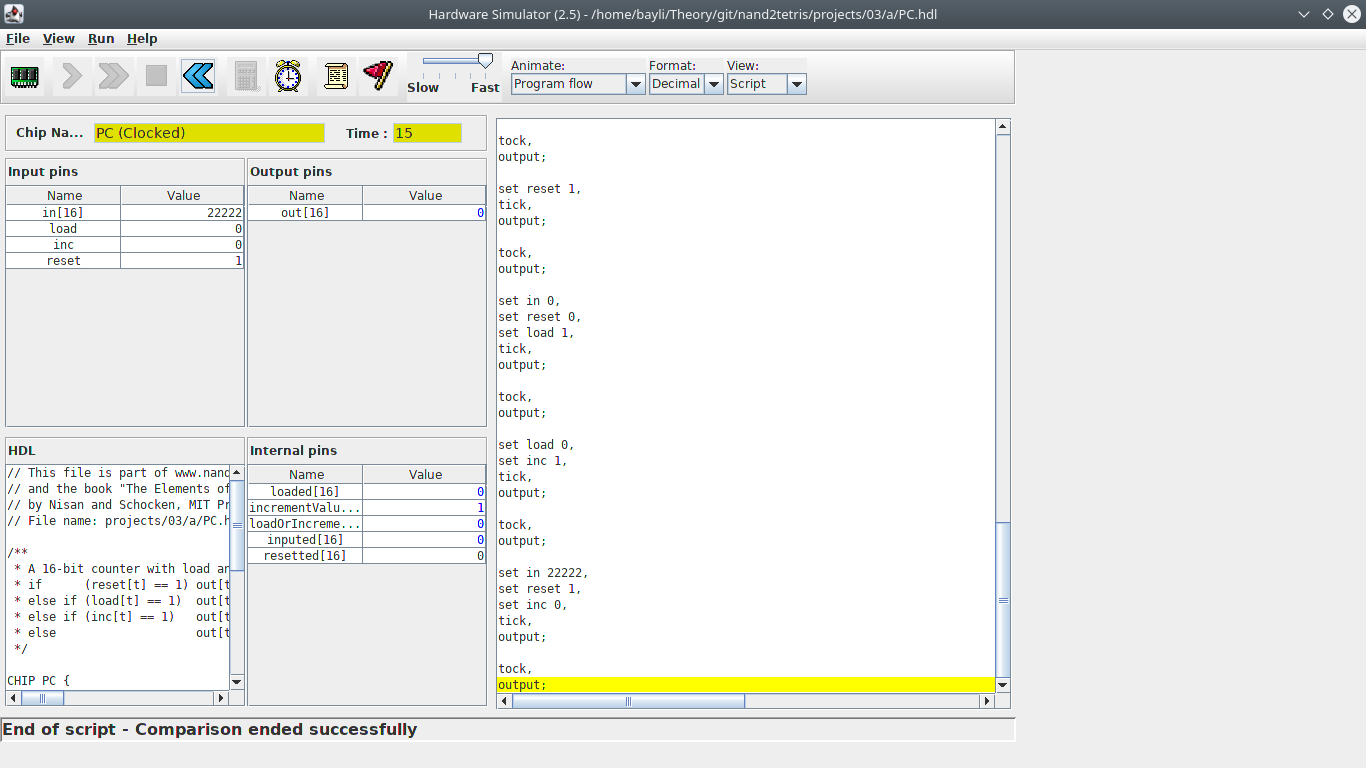
\includegraphics[width=.9\textwidth]{a/PC.png}
      }
    \end{description}
  }
  \item[b)]{
    \begin{description}
      \item[RAM512]{
        All test passed

        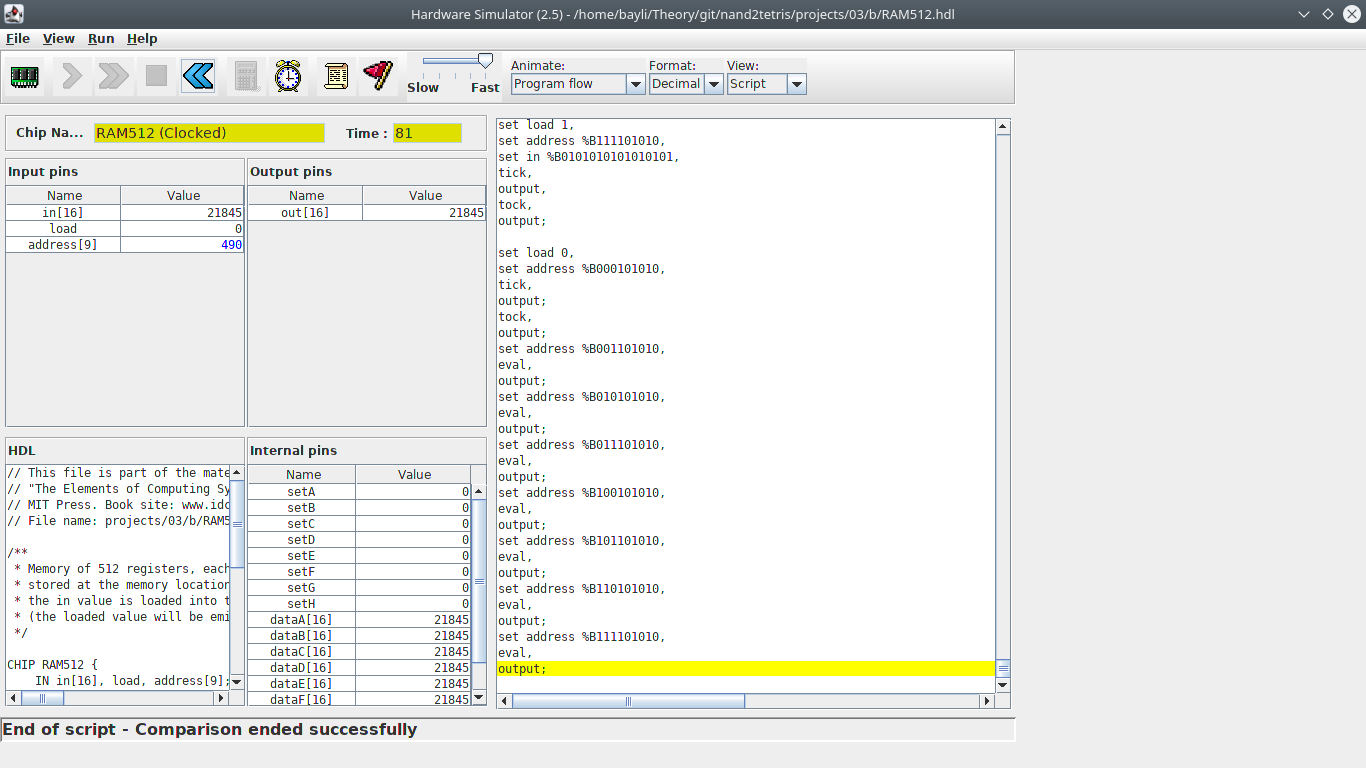
\includegraphics[width=.9\textwidth]{b/RAM512.png}
      }
      \item[RAM4K]{
        All test passed

        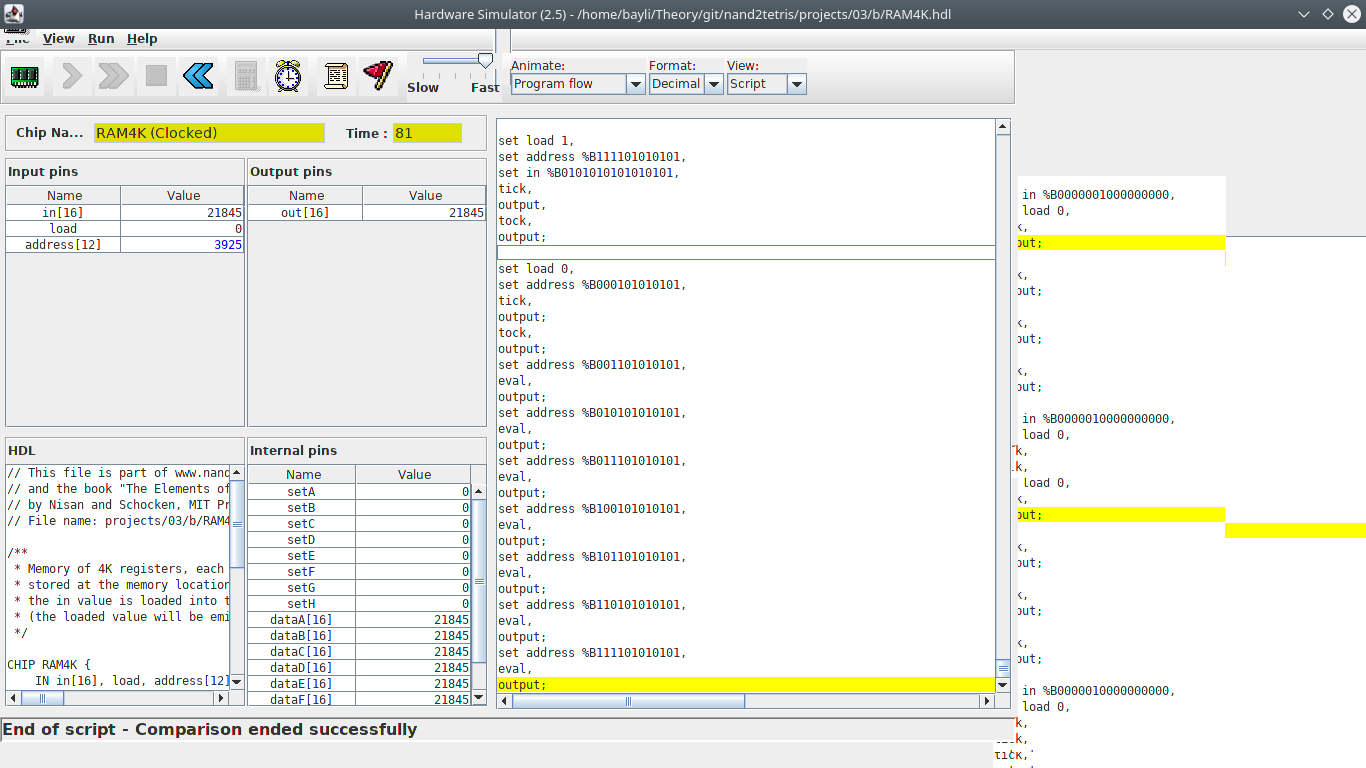
\includegraphics[width=.9\textwidth]{b/RAM4K.png}
      }
      \item[RAM16K]{
        All test passed

        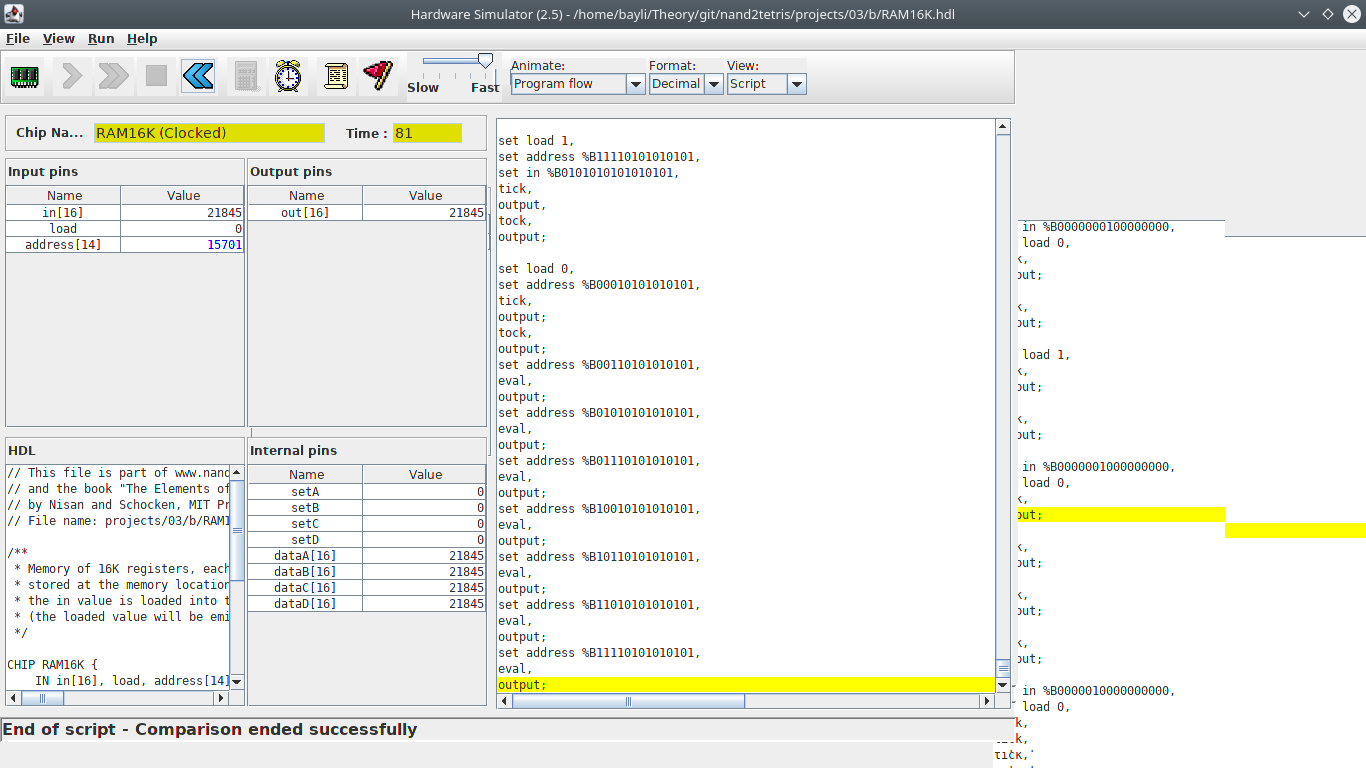
\includegraphics[width=.9\textwidth]{b/RAM16K.png}
      }
    \end{description}
  }
\end{enumerate}

All documenting of whether a test file is adequite is at the top of each .tst file

\end{document}